% To rebuild the .pdf from this source, use something like the following
%	latex quickref.tex
%	dvips -t letter -f < quickref.dvi >| quickref.ps
%	ps2pdf -sPAPERSIZE=letter quickref.ps
\documentclass[12pt]{article}
\usepackage[latin1]{inputenc}
\usepackage{lscape}
\usepackage{setspace}
\usepackage{graphicx}
\usepackage{multicol}
\usepackage[normalem]{ulem}
\usepackage[english]{babel}
\usepackage{color}
\usepackage{hyperref}

\textheight=9in
\textwidth=7.5in
\headheight=0pt
\headsep=0pt
\topmargin=0in
\oddsidemargin=-0.4in
\evensidemargin=-0.6in
\parindent=0pt
\parsep=1pt
\pagestyle{empty}

\date {}

\makeatother

\begin{document}
	\begin{landscape}

%	\textit{Dan Kuester's all-leather}

	\begin{center}
	\begin{minipage}[m]
		{1in}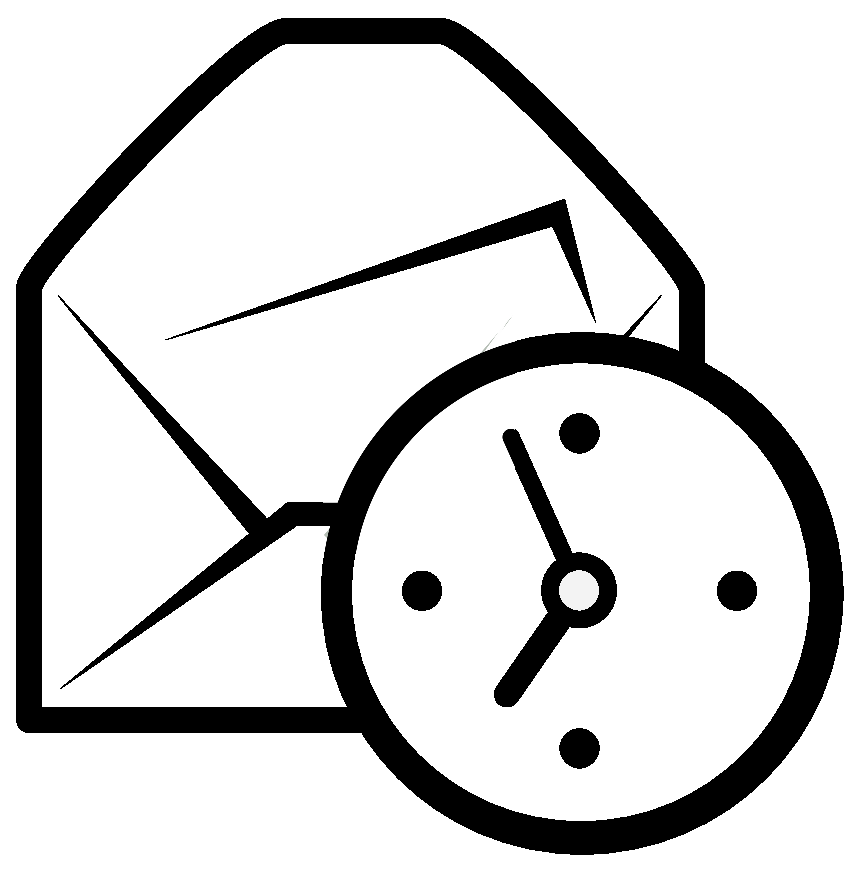
\includegraphics[height=0.9in]{../evolution-logo.eps}\hspace{5mm}
	\end{minipage}
	\hspace{5mm}
	\textbf{\Huge{Refer�ncia R�pida do Evolution}}
	\end{center}

	\begin{center}
	\begin{multicols}{2}
	\section*{Global}
	\begin{tabular*}{4in}{rp{1.5in}}
		\textit{\textbf{Componentes}}		&					\\
		Email					& \textbf{Ctrl+1}			\\
		Contactos				& \textbf{Ctrl+2}			\\
		Calend�rios				& \textbf{Ctrl+3}			\\
		Tarefas					& \textbf{Ctrl+4}			\\
		\vspace{1.5mm}
		Memos					& \textbf{Ctrl+5}			\\
		\textit{\textbf{Controlos}}		&					\\
		Novo item no modo actual		& \textbf{Ctrl+N}			\\
		Ciclar o foco entre paineis		& \textbf{F6}				\\
		Limpar a barra de procura		& \textbf{Shift+Ctrl+Q}			\\
		Fechar a janela				& \textbf{Ctrl+W}			\\
		Abrir uma nova janela			& \textbf{Shift+Ctrl+W}			\\
		\vspace{1.5mm}
		Sair do evolution			& \textbf{Ctrl+Q}			\\
		\textit{\textbf{Selec��o}}		&					\\
		Imprimir a selec��o			& \textbf{Ctrl+P}			\\
		Gravar a selec��o			& \textbf{Ctrl+S}			\\
		Apagar a selec��o			& \textbf{Del} or \textbf{Backspace}	\\
		Mover correio/contactos para a pasta	& \textbf{Shift+Ctrl+V}			\\
		Copiar correio/contactos para a pasta	& \textbf{Shift+Ctrl+Y}			\\
	\end{tabular*}
	\section*{Contactos/Componentes dos Memos}
	\begin{tabular*}{4in}{rp{1.5in}}
		\textit{\textbf{Comandos Gerais}}	&					\\
		Novo contacto				& \textbf{Shift+Ctrl+C}			\\
		Nova lista de contactos			& \textbf{Shift+Ctrl+L}			\\
		Novo memo				& \textbf{Shift+Ctrl+O}			\\
	\end{tabular*}
%	{\\ \vspace{5mm} \footnotesize \textit{* denotes the feature may not be implemented yet}}
	\section*{Componente de Email}
	\begin{tabular*}{4in}{rp{1.5in}}
		\textit{\textbf{Comandos Gerais}}	&					\\
		Nova mensagem				& \textbf{Shift+Ctrl+M}			\\
		\vspace{1.5mm}
		Enviar/Receber mensagens		& \textbf{F12}				\\
		\textit{\textbf{Selec��o}}		&					\\
		Aplicar filtros				& \textbf{Ctrl+Y}			\\
		Abrir numa nova janela 			& \textbf{Return} or \textbf{Ctrl+O}	\\
		\vspace{1.5mm}
		Reencaminhar a selec��o			& \textbf{Ctrl+F}			\\
		\textit{\textbf{Painel de Lista de Mensagens}}&					\\
		Mensagem por ler seguinte		& \textbf{.} or \textbf{]}		\\
		\vspace{1.5mm}
		Mensagem por ler anterior		& \textbf{,} or \textbf{[}		\\
		\textit{\textbf{Painel de Antevis�o}}	&					\\
		Responder ao remetente			& \textbf{Ctrl+R}			\\
		Responder para a lista			& \textbf{Ctrl+L}			\\
		Responder a todos os destinat�rios	& \textbf{Shift+Ctrl+R}			\\
		Rolar acima				& \textbf{Backspace}			\\
		Rolar abaixo				& \textbf{Space}			\\
	\end{tabular*}
	\section*{Componentes de Calend�rio/Tarefas}
	\begin{tabular*}{4in}{rp{1.5in}}
		\textit{\textbf{Comandos Gerais}}	&					\\
		Novo compromisso			& \textbf{Shift+Ctrl+A}			\\
		Nova reuni�o				& \textbf{Shift+Ctrl+E}			\\
		\vspace{1.5mm}
		Nova tarefa				& \textbf{Shift+Ctrl+T}			\\
%		\vspace{1.5mm}
%		Expunge/Purge old schedules		& \textbf{Ctrl+E}			\\
		\textit{\textbf{Navega��o}}		&					\\
		Ir para hoje				& \textbf{Ctrl+T}			\\
		Ir para a data				& \textbf{Ctrl+G}			\\
	\end{tabular*}
	\end{multicols}
	\end{center}
	\end{landscape}
 \end{document}
